\subsection{Architettura generale}

\subsubsection{Schema}
\begin{figure}[H]
    \centerfloat
    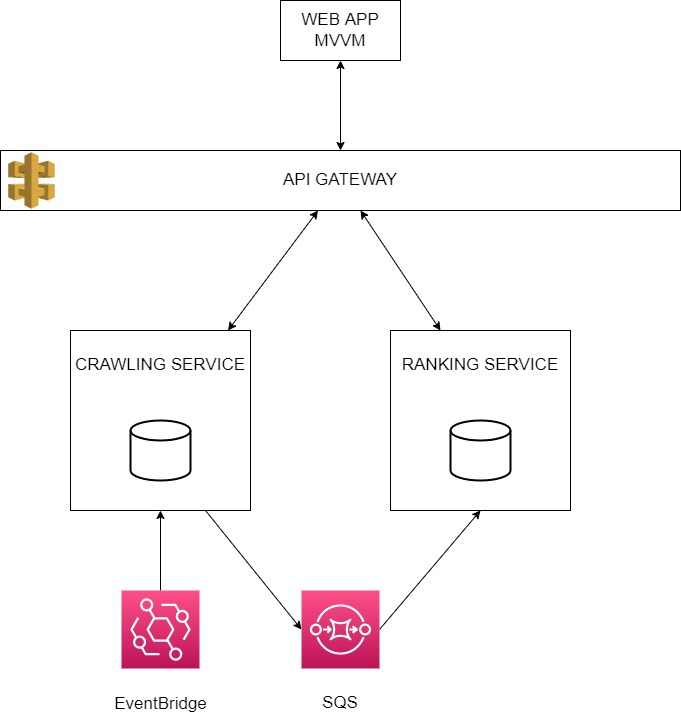
\includegraphics[scale=0.35]{Contenuto/Immagini/backend-architettura.jpg}
    \caption{Architettura generale}
\end{figure}

\subsubsection{Descrizione}
Come richiesto dal capitolato si è deciso di utilizzare un'architettura a microservizi, i quali comunicano con il Frontend tramite API Gateway\glo.
In particolare sono stati individuati i seguenti microservizi:
\begin{itemize}
    \item \textit{Crawling Service}: questo microservizio si occupa di tutto ciò che riguarda il crawling dei dati da Instagram. Il processo di crawling viene innescato da un servizio di AWS chiamato EventBridge\glo che si occupa dello scheduling del crawling. Ogni volte che viene trovato dal crawler un post relativo ad un ristorante, questo viene inviato ad una coda SQS\glo dalla quale andrà a leggere il servizio di ranking. Infine il Crawling Service espone una API al Frontend per permettere di suggerire profili Instagram da aggiungere alla lista di quelli osservati dal crawler.
    \item \textit{Ranking Service}: questo microservizio invece si occupa dell'analisi dei contenuti estratti dal crawler e della realizzazione di una classifica di ristoranti. Il processo di analisi di un post viene fatto partire dalla ricezione di un messaggio sulla coda SQS, una volta letto il messaggio esso viene rimosso dalla coda ed analizzato. Infine il Ranking Service espone molteplici API al Frontend in grado di fornire tutte le informazioni necessarie per poter visualizzare la classifica, i dettagli di un locale e la gestione dei preferiti.
\end{itemize}

Invece, per il Frontend è stato scelto di realizzare la struttura sfruttando il pattern architetturale \textit{Model-View-ViewModel} (MVVM), il quale comunica con il Backend esclusivamente tramite API Gateway.

Possiamo riassumere le motivazioni per cui abbiamo scelto il pattern architetturale MVVM per la parte Frontend come segue:

\begin{itemize}
\item La parte di Front-end è stata realizzata sfruttando la libreria React\glo che si integra particolarmente bene con il pattern MVVM,
\item Permette di riutilizzare i vari componenti in diversi contesti senza dover effettuare modifiche; un esempio è il modello che sfruttiamo per estrarre dati dal database, i quali (tramite la stessa chiamata) vengono usati in diverse pagine della WebApp. Lo stesso vale per la vista (perché usiamo un componente in diverse pagine della WebApp),
\item Permette di disaccoppiare la parte di business logic dalla presentation logic, aspetto che rende più semplice anche i test di unità,
\item Maggior semplicità di sviluppo in team: in questo modo, ogni singolo componente del gruppo può occuparsi di una sola parte della WebApp,
\item Manutenibilità più semplice, per via del disaccoppiamento del codice.
\end{itemize}
Inoltre, per la parte di autenticazione è stato utilizzato Cognito\glo, un servizio di AWS consigliatoci dall'azienda \textit{Zero12}, che permette di creare e gestire bacini d'utenza, oltre al framework AWS Amplify\glo per la parte di hosting ed autenticazione lato Frontend.

\subsubsection{Impostazioni coda SQS}
Per implementare la comunicazione tra microservizi è stata impostata una coda SQS, un servizio di accodamento messaggi 

